\documentclass[a4paper,12pt]{extarticle}
\usepackage[utf8]{inputenc}
\usepackage{polski}
\usepackage{biblatex}
\usepackage{graphicx}
\usepackage{listings}
\usepackage{hyperref}

\graphicspath{{./plots/pochmara-patryk} {./plots/rudnik-jakub} {./plots/sarwinski-wojciech}}
\addbibresource{bibliography.bib}

\renewcommand{\figurename}{Wykres}

\title{Projekt REGE - pomiar sygnałów}
\author{Pochmara Patryk 320727\\Rudnik Jakub 320731\\Sarwiński Wojciech 292863}
\date{24 marzec 2022}

\begin{document}

\maketitle

\begin{abstract}
Raport dotyczący pomiaru sygnałów, stanowiący część projektu stworzenia oprogramowania rozpoznającego płeć w oparciu o nagrania audio. Jest to semestralny projekt z podstaw teorii informacji wykorzystujący narzędzia stworzone w języku Python3. Jego celem jest stworzenie wydajnego algorytmu rozpoznającego płeć, przy użyciu algorytmów opracowanych na podstawie ręcznie przygotowanych danych.
\end{abstract}

\renewcommand{\abstractname}{Podział pracy}
\begin{abstract}
\noindent
Pochmara Patryk - \hyperref[sec:akwizycja]{Symulacja akwizycji sygnałów}\\
Sarwiński Wojciech - \hyperref[sec:aliasing]{Próbkowanie i efekty aliasingu}\\
Rudnik Jakub - \hyperref[sec:jakosc]{Porównywanie i ocena jakości sygnałów}\\
Cały kod dostępny jest w \href{https://github.com/zeraye/rege}{publicznym repozytorium}.
\end{abstract}

\newpage

\tableofcontents

\newpage

\section{Symulacja akwizycji sygnałów}
\label{sec:akwizycja}

Na potrzeby projektu niezbędne są próbki głosów damskich oraz męskich. Istotnym jest spostrzeżenie, że głos może być trudny do rozpoznania nawet dla człowieka, co może oznaczać, że algorytm będzie musiał brać pod uwagę subtelności głosu ludzkiego a nie wyłącznie częstotliwość. Co więcej zakłócenia wynikające z różnych form kompresji dźwięku dodatkowo utrudniają rozpoznanie płci mówiącego (więcej o tym w dalszej części raportu). Dlatego ważne było byśmy zdobyli zróżnicowane próbki na których oprzemy nasze wnioski i rozwiązania.

\newpage
    
\addcontentsline{toc}{section}{Narzędzia}
\section*{Narzędzia}

Do pomiaru sygnału wykorzystaliśmy programy Audacity i Dyktafon w zależności od tego czy nagranie dokonywane było na komputerze, czy na smartphone’ie. Oba nagrywają dźwięk z częstotliwością próbkowania 44100Hz. Audacity nagrywa sygnał dokładnie, czyli bez redukcji szumów ani innych rodzajów korekty. Dyktafon wykorzystuje pewne metody redukcji szumów otoczenia, by wychwycić głos mówiącego, jednak zmiany te nie wpływają znacząco na wyniki naszej analizy, a wręcz mogą ją ułatwić. Dokładne porównanie obu znajduje się w dalszej części raportu.

\begin{figure}[ht]
\centering
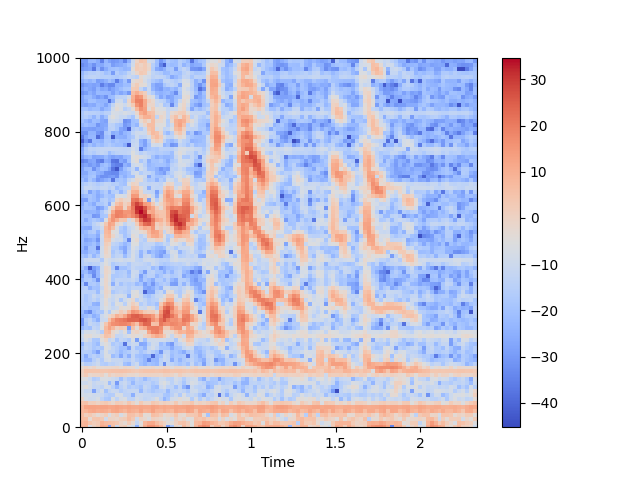
\includegraphics[width=0.6\textwidth]{1_female-audacity-normal-102.png}
\caption{ Spektrogram nagrania female-audacity-normal-102.wav}
\end{figure}

\begin{figure}[ht]
\centering
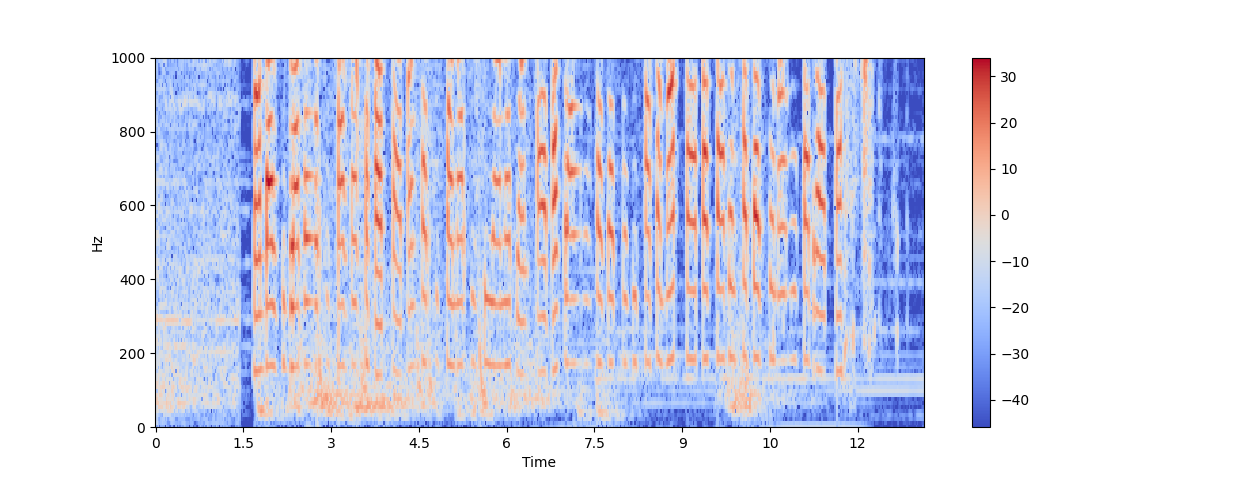
\includegraphics[width=0.6\textwidth]{1_male-discord-normal-101.png}
\caption{ Spektrogram nagrania male-discord-normal-101.wav}
\end{figure}

\newpage
       
\addcontentsline{toc}{section}{Miejsce / Źródło}
\section*{Miejsce / Źródło}

Pomiary, które wykonaliśmy pochodzą zarówno bezpośrednio od ochotników, jak i ochotników nagrywanych przez Internet, co wprowadza zniekształcenia wynikające z kompresji i algorytmów redukujących szumy. Próbki głosu gromadziliśmy z następujących źródeł:

\begin{itemize}
    \item Osobiście – nagranie smartphonem
    \item Osobiście – nagranie mikrofonem komputera
    \item Discord (komunikator głosowy VoIP)
    \item Twitch (platforma do nadawania na żywo)
    \item Youtube (platforma do publikowania filmów)
\end{itemize}

Wszystkie mają one swoje charakterystyki, dokładniej omówione dalej, ale większość nagrań jest dostatecznej jakości by człowiek był w stanie rozpoznać płeć mówiącego, co sugeruje że algorytm wykonujący te zadanie jest możliwy do utworzenia.

\begin{figure}[ht]
\centering
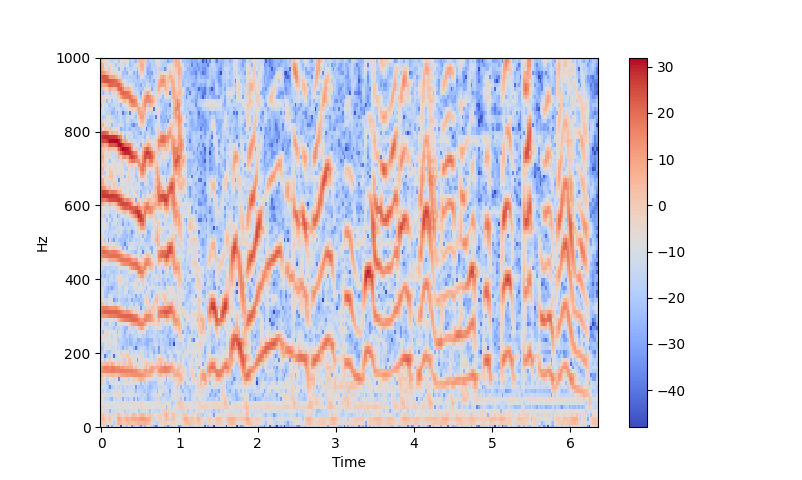
\includegraphics[width=0.5\textwidth]{2_male-twitch-normal-0.png}
\caption{ Spektrogram nagrania male-twitch-normal-0.wav}
\end{figure}

\begin{figure}[ht]
\centering
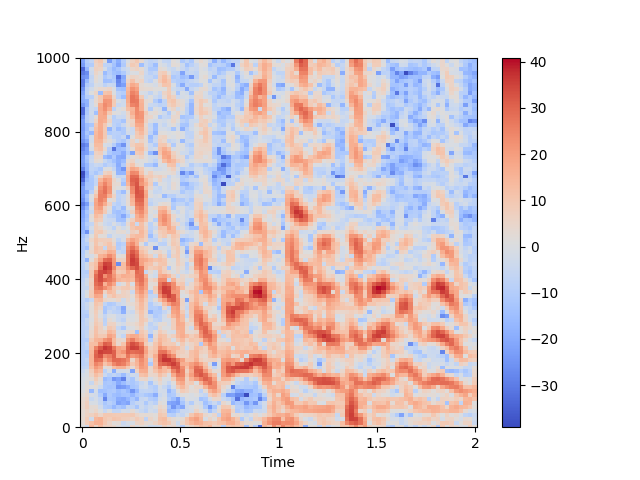
\includegraphics[width=0.5\textwidth]{2_male-youtube-normal-0.png}
\caption{ Spektrogram nagrania male-youtube-normal-0.wav}
\end{figure}

\newpage

\addcontentsline{toc}{section}{Warunki}
\section*{Warunki}

Skutkiem dużej liczby pomiarów są także odchylenia w warunkach, które panowały podczas nagrywania. Np. próbkom z uczelni towarzyszy szum rozmów w tle, a te nagrane na komputerze zawierają buczenie o niskiej częstotliwości (defekt mikrofonu), które podczas analizy widma mogą zmylić zarówno człowieka jak i algorytm. Kwestia warunków jest szczególnie ważna podczas tworzenia algorytmu, ponieważ jest to jeden z dwóch aspektów, których nasz program z zaimplementowanym algorytmem rozpoznawania płci nie będzie mógł kontrolować. Kluczowe jest więc by był on jak najmniej na nie wrażliwy i potrafił odfiltrować informację.

\begin{figure}[ht]
\centering
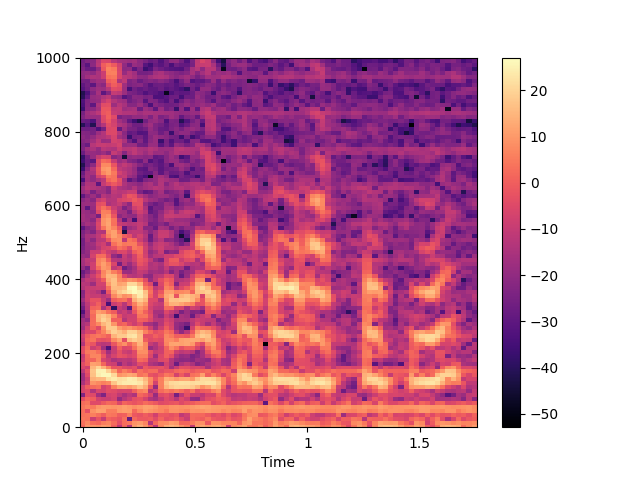
\includegraphics[width=0.55\textwidth]{3_male-audacity-normal-100.png}
\caption{ Spektrogram nagrania male-audacity-normal-100.wav}
\end{figure}

\begin{figure}[ht]
\centering
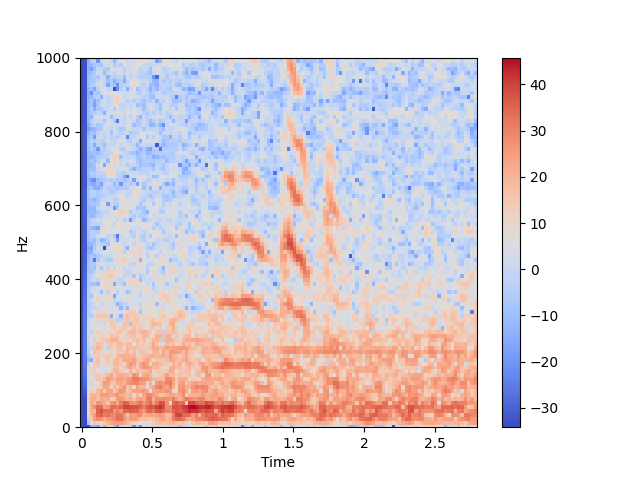
\includegraphics[width=0.55\textwidth]{3_male-iphone-normal-100.png}
\caption{ Spektrogram nagrania male-iphone-normal-100.wav}
\end{figure}

\newpage

\addcontentsline{toc}{section}{Płeć}
\section*{Płeć}

Najważniejszą różnicą w zebranych próbkach jest płeć mówiącego, jako że jej zgadnięcie jest celem algorytmu. Wyraźnie widać różnicę między pierwszą harmoniczną głosu mężczyzny i kobiety. Należy jednak zaznaczyć, że poniższe widma są spektrogramem nagrań, w których poprosiliśmy ochotników by mówili normalnym głosem przez około 2 sekundy ‘A’ (jak u dentysty). Pozostałe przypadki opisane są w kolejnych podsekcjach.

\begin{figure}[ht]
\centering
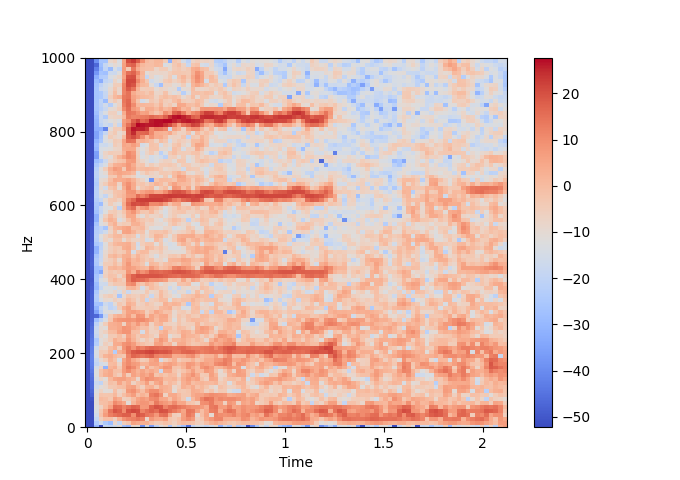
\includegraphics[width=0.6\textwidth]{4_female-iphone-normal-102.png}
\caption{ Spektrogram nagrania female-iphone-normal-102.wav}
\end{figure}

\begin{figure}[ht]
\centering
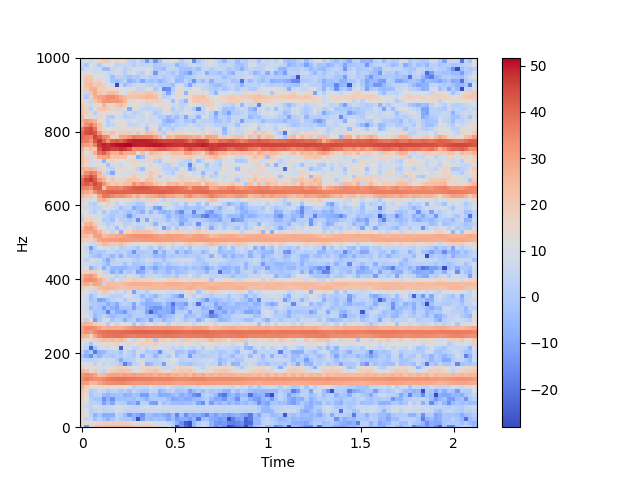
\includegraphics[width=0.6\textwidth]{4_male-discord-normal-2.png}
\caption{ Spektrogram nagrania male-discord-normal-2.wav}
\end{figure}

\newpage

\addcontentsline{toc}{section}{Modulacja głosu}
\section*{Modulacja głosu}

Interesującym odkryciem podczas wstępnej analizy próbek było spostrzeżenie, że modulacja głosu mówiącego jest istotnym czynnikiem, który znacząco wpływa na widmo częstotliwości głosu. Próba mówienia „niskim głosem” obniża pierwszą harmoniczną o zaledwie kilka (rzadko kilkanaście) Hz. Nie jest to więc problem. Za to mówienie „wysokim” czy też piskliwym głosem potrafi kompletnie uniemożliwić rozpoznanie płci człowiekowi, a co za tym idzie wymagało by od algorytmu innego rodzaju analizy, jeśli w ogóle jakaś byłaby w stanie dostarczyć informacji o płci mówiącego.

\begin{figure}[ht]
\centering
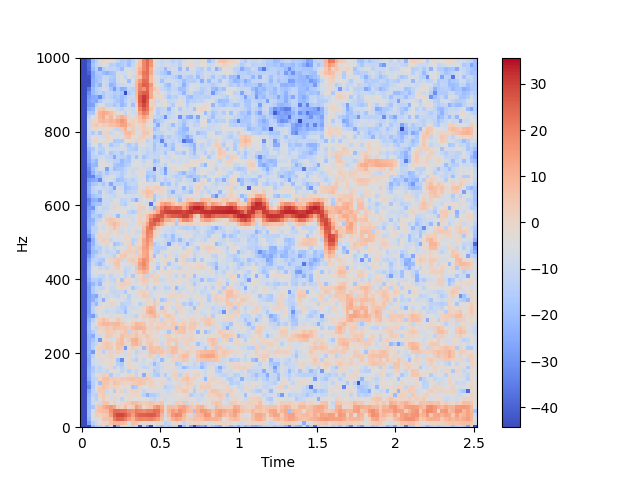
\includegraphics[width=0.6\textwidth]{5_female-iphone-high-102.png}
\caption{ Spektrogram nagrania female-iphone-high-102.wav}
\end{figure}

\begin{figure}[ht]
\centering
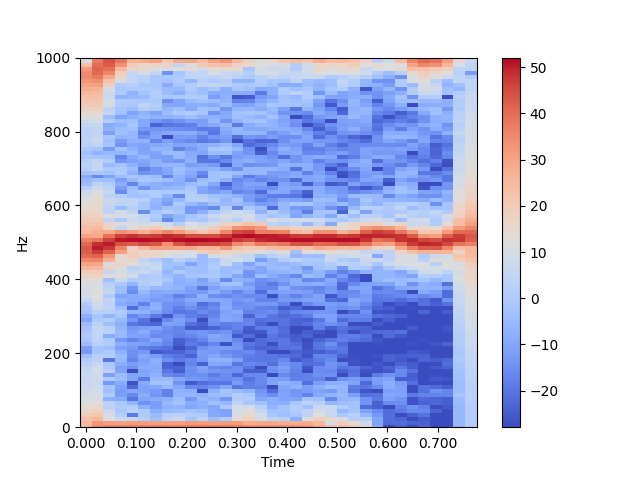
\includegraphics[width=0.6\textwidth]{5_male-discord-high-1.png}
\caption{ Spektrogram nagrania male-discord-high-1.wav}
\end{figure}

\newpage

\addcontentsline{toc}{section}{Charakterystyka mowy}
\section*{Charakterystyka mowy}

Częstotliwość głosu najłatwiej odczytać, gdy próbka zawiera pojedynczą głoskę. Np. ‘A’ trzymane przez 2 sekundy jak u dentysty. Jednak mowa ludzka jest znacznie bardziej skomplikowana i na widmie częstotliwości wyraźnie widać, że pierwsza harmoniczna waha się w pewnym przedziale. Te wahania algorytm będzie musiał brać pod uwagę, ponieważ są one wystarczająco duże by mężczyzna przez chwilę wszedł w zakres kobiet. Jednak najniższe punkty krzywych znajdują się zawsze w odpowiednim przedziale.

\begin{figure}[ht]
\centering
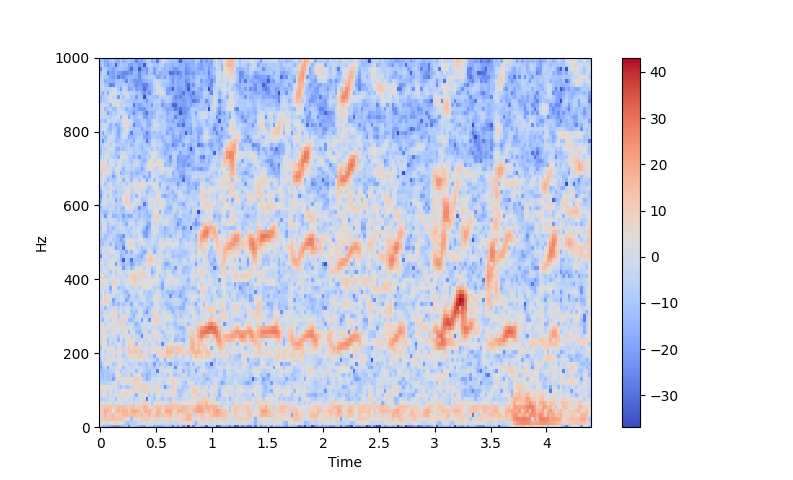
\includegraphics[width=0.6\textwidth]{6_female-iphone-normal-103.png}
\caption{ Spektrogram nagrania female-iphone-normal-103.wav}
\end{figure}

\begin{figure}[ht]
\centering
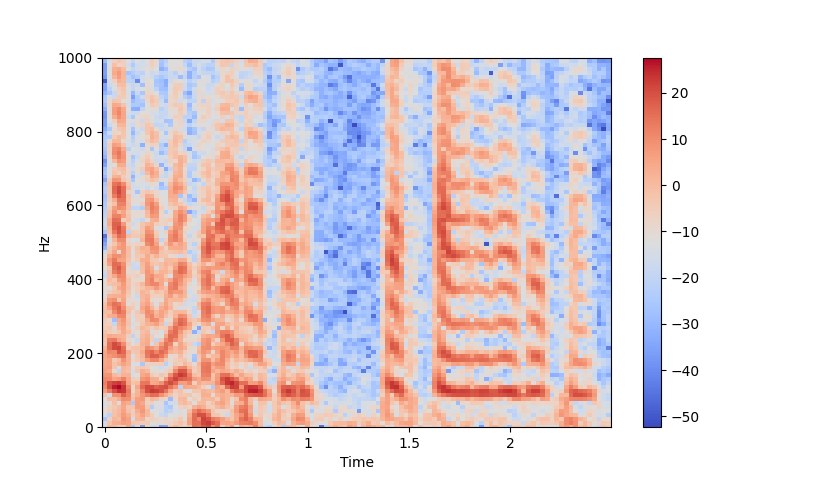
\includegraphics[width=0.6\textwidth]{6_male-discord-normal-3.png}
\caption{ Spektrogram nagrania male-discord-normal-3.wav}
\end{figure}

\newpage

\addcontentsline{toc}{section}{Wiek}
\section*{Wiek}

Ostatnim ważnym czynnikiem w głosie jest wiek mówiącego. Niestety zdecydowana większość próbek jakimi dysponujemy pochodzi od osób w wieku 18 – 60, więc dane dotyczące pozostałych przedziałów wiekowych są ograniczone. Dla małych dzieci głosy mogą być wręcz nierozróżnialne, co wynika z faktu braku zmian zachodzących w organizmie w okresie dojrzewania. Do czasu mutacji głos chłopaka może okazać się być problematyczny do jednoznacznego określenia. Natomiast dla starszych osób różnica jest wyraźnie słyszalna dla człowieka, co pozwala wnioskować, że będzie także widoczna dla algorytmu.

\newpage

\section{Próbkowanie i efekty aliasingu}
\label{sec:aliasing}

W tej sekcji raportu omówione zostanie próbkowanie sygnału i wpływ częstotliwości próbkowania na efekt aliasingu w kontekście zapisywania dźwięku.
       
\addcontentsline{toc}{section}{Próbkowanie}
\section*{Próbkowanie}

Próbkowanie to proces służący do stworzenia reprezentacji sygnału ciągłego w postaci sygnału dyskretnego. Sygnał dyskretny reprezentuje sygnał analogowy za pomocą ciągu wartości nazywanych próbkami. Sygnał dyskretny \(f_s(t)\) otrzymujemy z iloczynu sygnału analogowego \(f(t)\) i funkcji próbkującej \(s(t)\).

\[f_s(t) = f(t) * s(t)\]

W idealnym przypadku funkcja próbkująca jest funkcją grzebieniową \(\delta(t)\), tzn. próbkowanie odbywa się w nieskończenie krótkim czasie.

\begin{figure}[h]
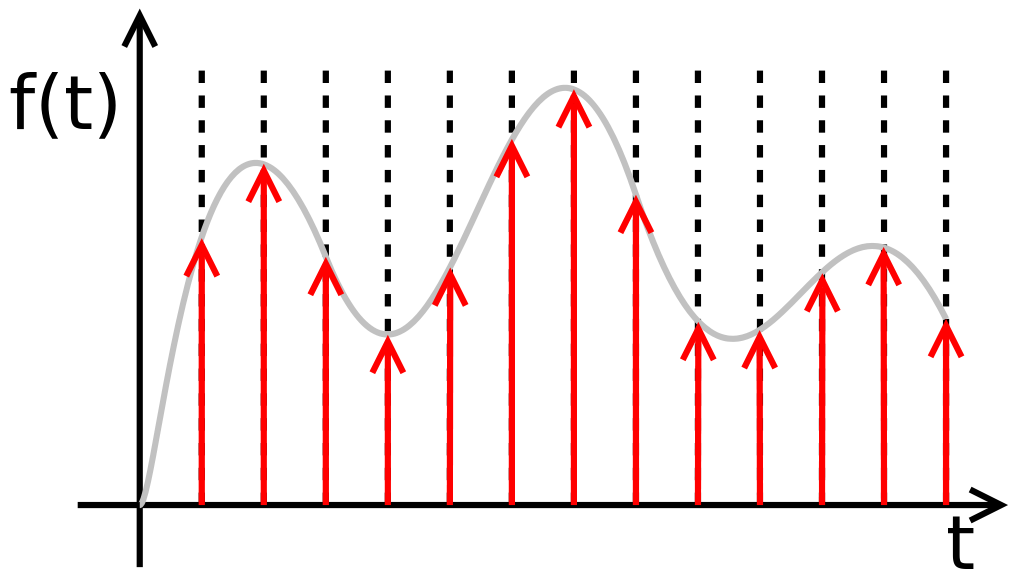
\includegraphics[height=4cm]{SampledSignal.png}
\centering
\caption{Próbkowanie sygnału w dziedzinie czasu}
\end{figure}

Przedstawiając sygnał w dziedzinie częstotliwości otrzymujemy widmo sygnału ciągłego. Po próbkowaniu możemy zauważyć, że sygnał spróbkowany ma charakter szeregu kopii widma oryginalnego przesuniętych od siebie o całkowite wielokrotności częstotliwość próbkowania.

Twierdzenie Nyquista-Shannona ustala, że można z sygnału dyskretnego \(f^*(t)\) złożonego z próbek sygnału ciągłego \(f(t)\) można wiernie odtworzyć sygnał \(x(t)\), jeśli widma sygnału oryginalnego i wszystkie jego kopie przesunięte o całkowite wielokrotności częstotliwości próbkowania nie nachodzą na siebie. Co oznacza, że częstotliwość próbkowania \(f_s\) musi być większa od dwukrotności granicznej wartości częstotliwości widma sygnału oryginalnego. Graniczną wartość częstotliwości próbkowania spełniająca to założenie jest nazywana częstotliwością Nyquista.

\begin{figure}[h]
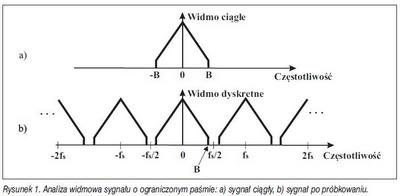
\includegraphics[height=5cm]{WidmaPor.jpg}
\centering
\caption{Widma sygnału a) ciągłego, b) po próbkowaniu \cite{JanErhard}}
\end{figure}

\newpage

\addcontentsline{toc}{section}{Aliasing}
\section*{Aliasing}

Aliasing jest to zjawisko, w którym sygnał powstały w procesie próbkowania zostaje nieodwracalnie zniekształcony. Aliasing występuje przy nakładaniu się kopii widm sygnałów ciągłych w widmie sygnału dyskretnego. Następuje to, gdy częstotliwość próbkowania \(f_s\) jest mniejsza od podwojonej granicznej wartości częstotliwości widma mierzonego sygnału, czyli gdy nie spoełnione jest twierdzenie Nyquista-Shannona, nazywane również twierdzeniem o próbkowaniu.

Efektem aliasingu dla sygnałów o częstotliwości wyższych od częstotliwości Nyquista dla danej częstotliwości próbkowania jest ich "odbicie", tzn. wraz z wzrostem częstotliwości sygnału jego częstotliwość po próbkowaniu zostanie zinterpretowana jako coraz niższa.

\begin{figure}[h]
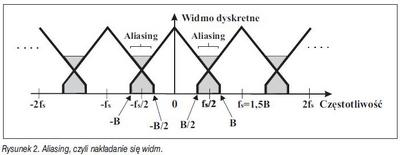
\includegraphics[height=5cm]{NachodzWidma.jpg}
\centering
\caption{Nakładające się widmo dyskretne po próbkowaniu \cite{JanErhard}}
\end{figure}

W celu uniknięcia efektów aliasingu należy najpierw dostosować częstotliwość próbkowania do potrzeb. Jeżeli mamy do przetworzenia sygnał dźwiękowy w przedziale słyszalnym dla ludzi tzn. od 20Hz do 20kHz, to możemy próbkować z częstotliwością większą niż 40kHz. Jeżeli zależy nam tylko na przekazaniu ludzkiej mowy możemy użyć częstotliwości tak niskiej jak 8kHz.

Dodatkowo, żeby uniknąć nakładania się widm, powinno zastosować się filtr antyaliasingowy. Filtr antyaliasingowy jest filtrem dolnoprzepustowym, to znaczy, że przepuszcza sygnały tylko o częstotliwości niższej od ustalonej częstotliwości granicznej i tłumi składowe widma o częstotliwości wyższej niż częstotliwość graniczna.


\newpage

\section{Porównywanie i ocena jakości sygnałów}
\label{sec:jakosc}

\addcontentsline{toc}{section}{Krótki opis sekcji}
\section*{Krótki opis sekcji}

W tej sekcji porównam jakość zebranych próbek nagrań w zależności od źródła z którego pochodzą. Jakość w mojej definicji oznacza łatwość określenia częstotliwości głosu autora nagrania. Najbardziej interesującą wartością będzie pierwsza harmoniczna, gdyż ona odpowiada za powszechnie uznawaną "częstotliwość głosu człowieka". Próbki w zależności od źródła pochodzenia podzieliłem na 5 części:

\begin{enumerate}
    \item Dyktafon iPhone
    \item Audacity
    \item Discord
    \item Twitch
    \item YouTube
\end{enumerate}

\addcontentsline{toc}{section}{Problem braku kodu źródłowego}
\section*{Problem braku kodu źródłowego}

Niestety jedynymi aplikacjami typu "open source" jest Discord i Audacity. Dzięki publicznemu kodu źródłowego, można sprawdzić sposoby kompresji i obróbki pliku dźwiękowego wpływające na jakość próbki. Algorytmy obórbki sygnałów dźwiękowych w pozostałych aplikacjach nie są jawne, więc bazować będę na różnych źródłach znalezionych w Internecie. Nie daje mi to gwarancji, że takowe rozwiązania są obecnie używane w tych aplikacjach, lecz mogą opisywać starsze wersje danych produktów.

\addcontentsline{toc}{section}{Porównywanie jakości sygnałów}
\section*{Porównywanie jakości sygnałów}

Porównywanie jakości sygnałów zostało podzielone na dwie części.

\begin{enumerate}
    \item W pierwszej (percepcyjnej) bazując na ręcznych odczytach ze spektrometru sprawdzę, które próbki zawierają najmniej zakłóceń, nie posiadają artefaktów oraz w sposób najbardziej jednoznaczny można określić częstotliwość głosu autora nagrania.

    \item W drugiej (obliczeniowej) korzystając z dalej przedstawionych algorytmów, porównam jakości sygnałów bazując na analizie spektrogramu. Algorytmiczna ocena jakości sygnałów również obarczona zostanie błędem, gdyż analizę złożonych struktur i danych niezwykle ciężko jest przeprowadzać za pomocą obliczeń maszynowych.
\end{enumerate}

Następnie przeanalizuję, który sposób oceny jakości sygnału został przeprowadzony bardziej rzetelnie. Takie badanie pokaże mi zalety i wady komputerowej analizy jakości sygnałów.

\addcontentsline{toc}{section}{Percepcyjne porównanie jakości sygnałów}
\section*{Percepcyjne porównanie jakości sygnałów}

Na początku podkreślę, że spektrogramy na których jest wyraźnie zarysowana prosta pozioma linia, są nagraniami w którym autor wymawiał pojedynczą samogłoskę. Z takich nagrań najłatwiej jest odczytać spektrum głosu. Wykresy o bardziej pofałdowanych wykresach prezentują słowa, które zniekształcają cały obraz.

\addcontentsline{toc}{section}{Dyktafon iPhone}
\section*{Dyktafon iPhone}

Jako pierwszej aplikacji przyjrzę się plikom dźwiękowym nagranym przy użyciu dyktafonu z iPhona.

\begin{figure}[h]
\centering
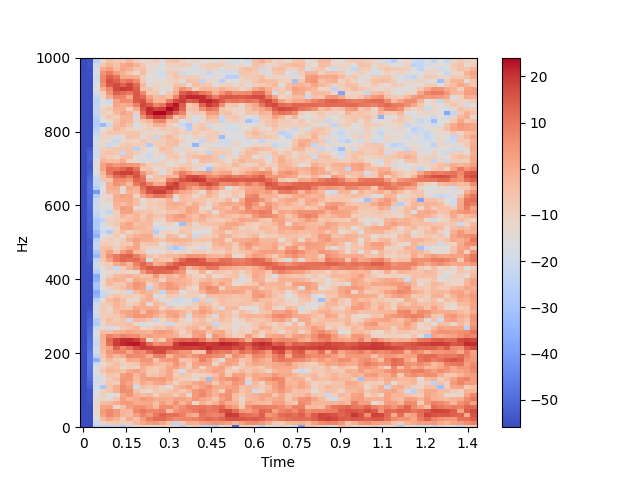
\includegraphics[width=0.6\textwidth]{iphone-0}
\caption{Spektrogram nagrania female-iphone-normal-100.wav}
\end{figure}

\newpage

\begin{figure}[h]
\centering
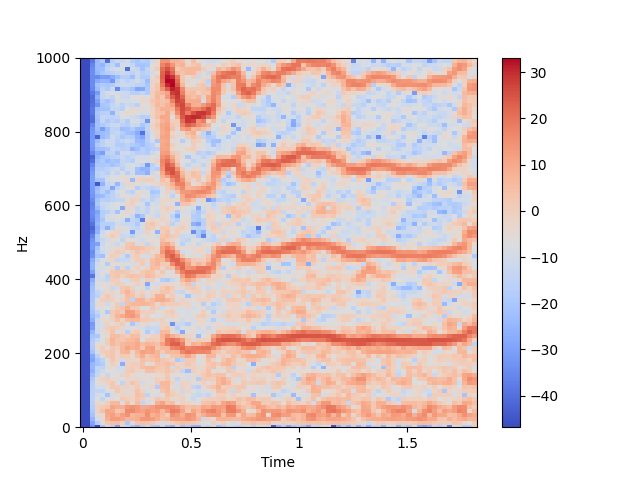
\includegraphics[width=0.6\textwidth]{iphone-1}
\caption{Spektrogram nagrania female-iphone-normal-101.wav}
\end{figure}

\begin{figure}[h]
\centering
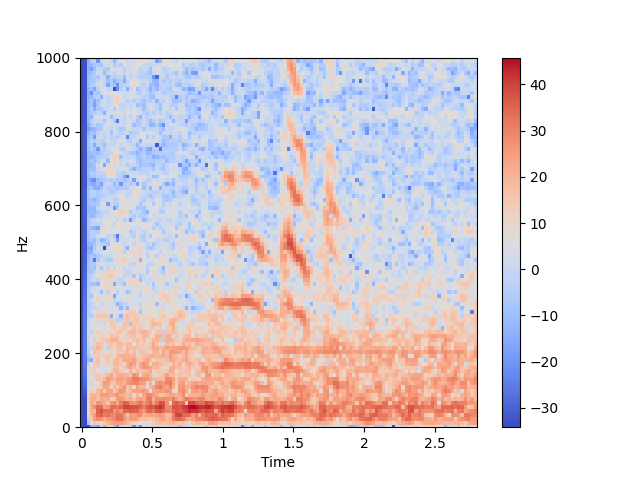
\includegraphics[width=0.6\textwidth]{iphone-2}
\caption{ Spektrogram nagrania male-iphone-normal-100.wav}
\end{figure}

\subsection*{}
Dla głosu kobiecego spektrum jest dość rozmyte, ale człowiek jest w stanie odczytać wartość pierwszej częstotliwości harmonicznej. Dla głosu męskiego, wykres jest zbyt zniekształcony, aby móc odczytać z niego cokolwiek. Całe spektrum poniżej 350 Hz jest całkowicie rozmyte i można tylko szacować możliwą częstotliwość przez miejsca, gdzie dźwięk jest najgłośniejszy (ciemnoczerwony kolor). Rozmycie wynika głównie z niskiej jakości nagrania.

\newpage

\addcontentsline{toc}{section}{Audacity}
\section*{Audacity}

Następnie sprawdzę jak wyglądają spektrogramy, wygenerowane z plików dźwiękowych nagranych bezpośrednio przez aplikację Audacity.

\begin{figure}[h]
\centering
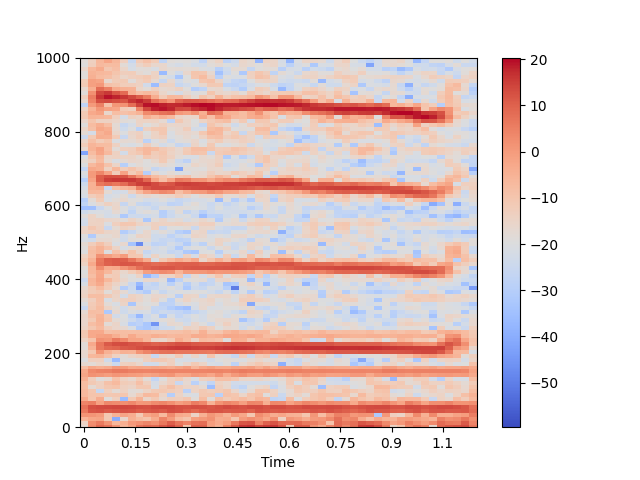
\includegraphics[width=0.6\textwidth]{audacity-0}
\caption{Spektrogram nagrania female-audacity-normal-100.wav}
\end{figure}

\begin{figure}[h]
\centering
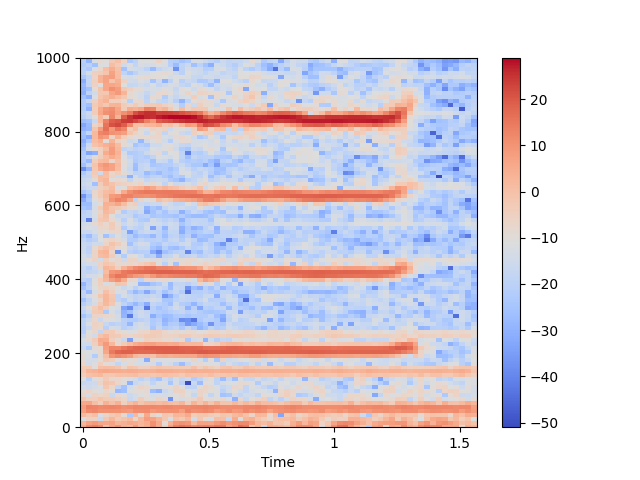
\includegraphics[width=0.6\textwidth]{audacity-1}
\caption{Spektrogram nagrania female-audacity-normal-101.wav}
\end{figure}

\newpage

\begin{figure}[h]
\centering
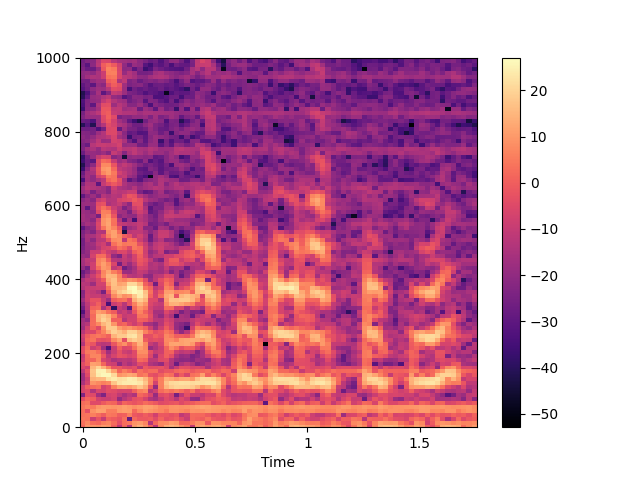
\includegraphics[width=0.6\textwidth]{audacity-2}
\caption{Spektrogram nagrania male-audacity-normal-100.wav}
\end{figure}

\subsection*{}
Tutaj niezwykle przejrzyście widać całe spektrum głosu. Odczytanie pierwszych harmonicznych jest bardzo proste. W wykresie \textbf{male-audacity-normal-100.wav} pojawia się artefakt w postaci pomarańczowej linii. Nie jest to pierwsza harmoniczna, lecz prawdopodobnie jakieś odgłosy tła. Dla mniej doświadczonego oka, może być on przyczyną źle odczytanej wartości. Warto zwrócić uwagę na to, że Audacity w żaden sposób nie filtruje danych, jeżeli wyraźnie tego nie włączymy (nagrania były bez filtrów). \cite{audacity}

\newpage

\addcontentsline{toc}{section}{Discord}
\section*{Discord}

Teraz przeanalizuję nagrania pobrane podczas rozmów w aplikacji Discord.

\begin{figure}[h]
\centering
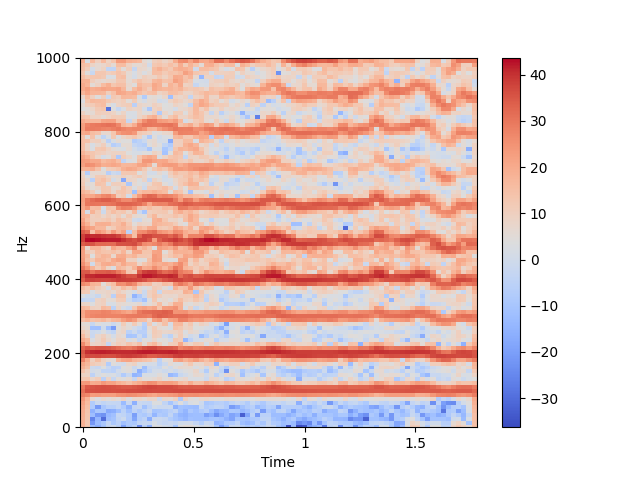
\includegraphics[width=0.6\textwidth]{discord-0}
\caption{Spektrogram nagrania male-discord-normal-0.wav}
\end{figure}

\begin{figure}[h]
\centering
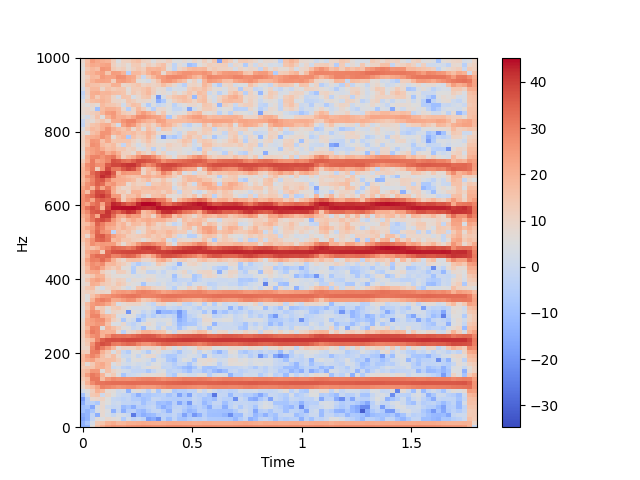
\includegraphics[width=0.6\textwidth]{discord-1}
\caption{Spektrogram nagrania male-discord-normal-1.wav}
\end{figure}

\begin{figure}[h]
\centering
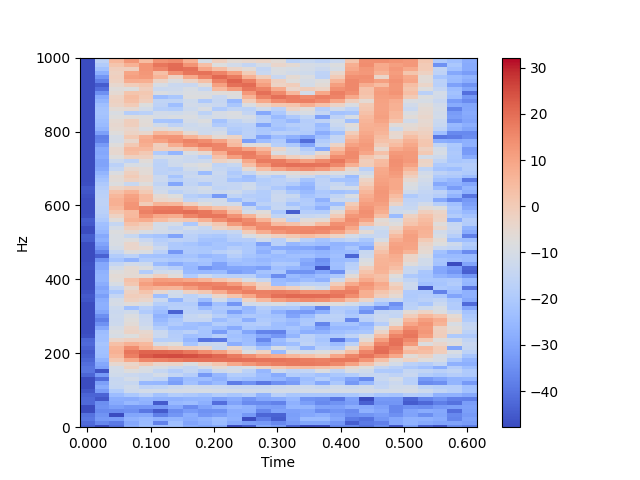
\includegraphics[width=0.6\textwidth]{discord-2}
\caption{Spektrogram nagrania female-discord-normal-100.wav}
\end{figure}

\newpage

\subsection*{}
Podobnie jak nagrania w Audiacity, wykresy są niezwykle czytelne. Problemem jest artefakt na wykresie \textbf{male-discord-normal-1.wav} Pozioma linia biegnąca w okolicach 0 Hz może stanowić problem dla algorytmu odczytującego pierwszą harmoniczną. Człowiek jest w stanie wyłapać ten problem i nie uznawać tej linii jako informacji. Wykres \textbf{female-discord-normal-100.wav} jest nieco gorszej jakości, wynika to z krótkiej długości nagrania. Nie stanowi to żadnego problemu w odczytaniu częstotliwości. \cite{discord}

\newpage

\addcontentsline{toc}{section}{Twitch}
\section*{Twitch}

Następnie nagrania zostały zdobyte z platformy Twitch. Mogą być one ciekawe, gdyż takie strony, gdzie ludzie występują na żywo mają złożone algorytmy kompresujące.

\begin{figure}[h]
\centering
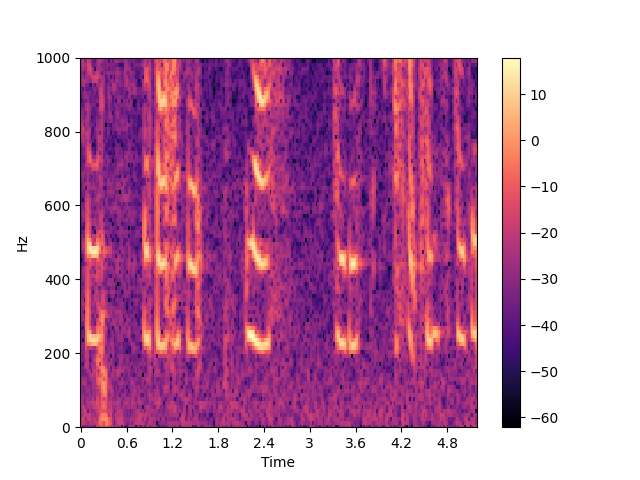
\includegraphics[width=0.6\textwidth]{twitch-0}
\caption{Spektrogram nagrania female-twitch-normal-0.wav}
\end{figure}

\begin{figure}[h]
\centering
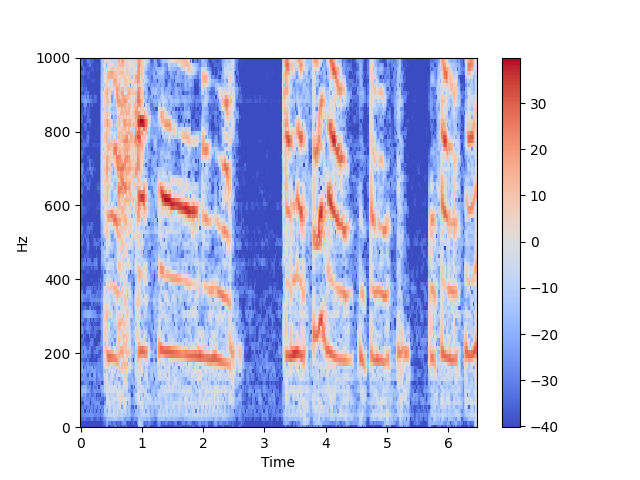
\includegraphics[width=0.6\textwidth]{twitch-1}
\caption{Spektrogram nagrania female-twitch-normal-1.wav}
\end{figure}

\begin{figure}[h]
\centering
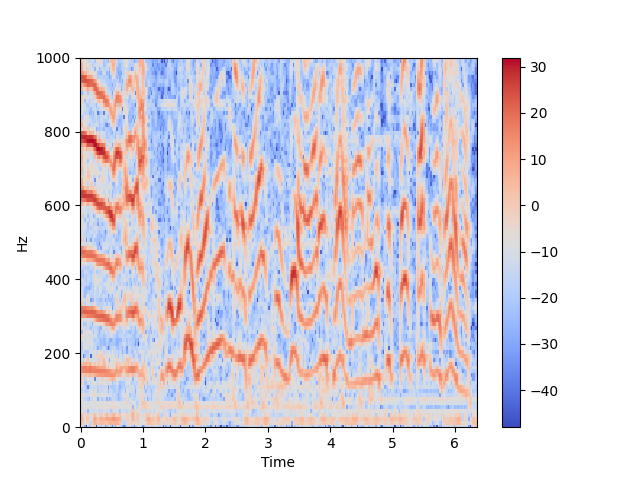
\includegraphics[width=0.6\textwidth]{twitch-2}
\caption{Spektrogram nagrania male-twitch-normal-0.wav}
\end{figure}

\newpage

\subsection*{}
Próbki pobrane z platformy Twitch, są dość dobrej jakości. Wyraźnie widać, że platforma używa filtrów, gdyż kolejne częstotliwości harmoniczne są wyraźnie podkreślone. Obszary pomiędzy nimi są wytłumione. Możemy również zauważyć, że są nałożone algorytmy całkowicie wyciszające w momentach kiedy nikt nic nie mówi. Dzięki temu usunięte są wszelkiego rodzaju szmery.

\newpage

\addcontentsline{toc}{section}{YouTube}
\section*{YouTube}

Jako ostatnie przeanalizuję jakość nagrań z największej platformy udostępniającej nagrania wideo YouTube. Nagrania zostały pobrane w najwyżej możliwej jakości.

\begin{figure}[h]
\centering
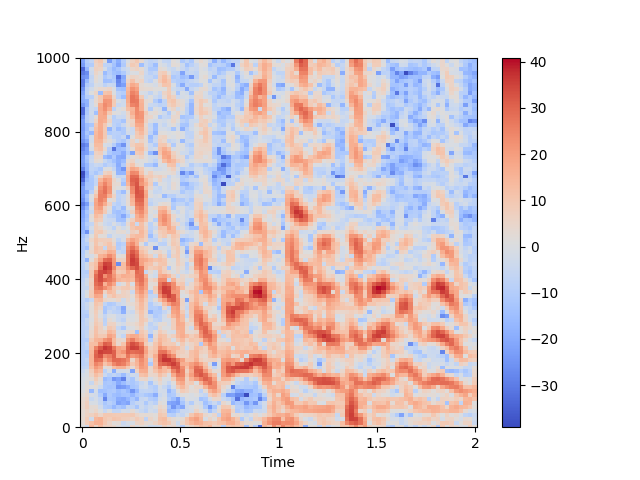
\includegraphics[width=0.6\textwidth]{youtube-0}
\caption{Spektrogram nagrania male-youtube-normal-0.wav}
\end{figure}

\begin{figure}[h]
\centering
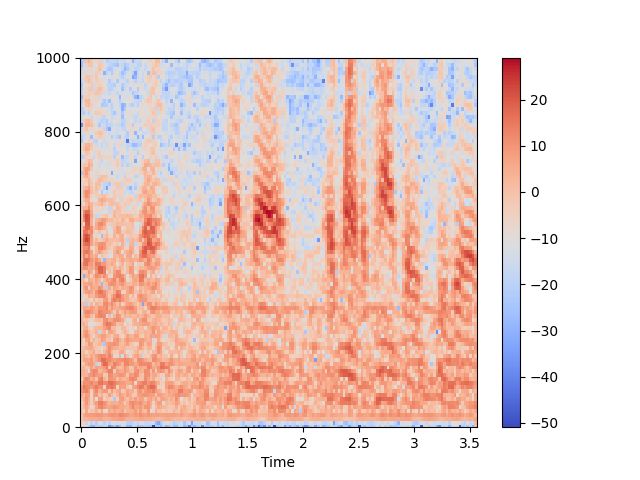
\includegraphics[width=0.6\textwidth]{youtube-1}
\caption{Spektrogram nagrania male-youtube-normal-4.wav}
\end{figure}

\begin{figure}[h]
\centering
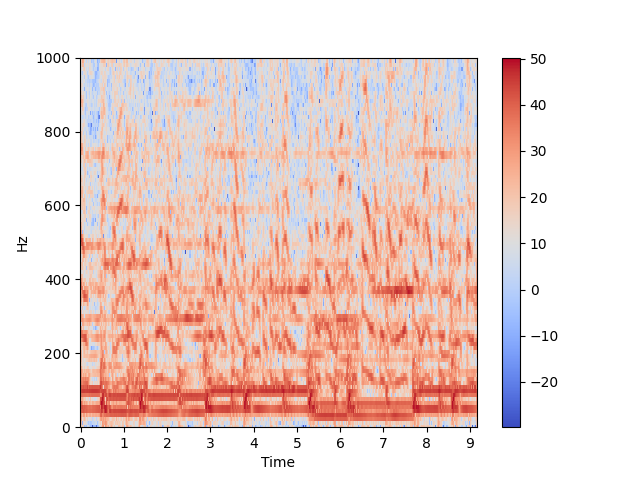
\includegraphics[width=0.6\textwidth]{youtube-2}
\caption{Spektrogram nagrania male-youtube-normal-5.wav}
\end{figure}

\newpage

\subsection*{}
Nagrania w większości są fatalnej jakości. Mamy tutaj do czynienia z silną kompresją. Znacząco wpływa ona na jakość dźwięku. Nagranie niemal idealnie czyste wykres \textbf{male-youtube-normal-0.wav} jest zniekształcone i ma trudny do wykrycia przez algorytm artefakt. Jest on w postaci pionowej linii co jest nie spotykane na innych spektrogramach (jeden ze spektrogramów z Twitcha miał podobną linie, lecz dużo bladszą). Trzeba dodatkowo uwzględnić ten problem przy przyszłym odczytywaniu pierwszej harmonicznej. Z pozostałych nagrań nie można jednoznacznie określić częstotliwości głosu autora nagrania. Wykresy \textbf{male-youtube-normal-4.wav} i \textbf{male-youtube-normal-5.wav} są rozmazane i widocznie przefiltrowane, aby zajmowały jak najmniej miejsca. Domyślam się, że taka platforma mająca prawdopodobnie miliony godzin nagrań, aby zapisać dane w sensownej ilości miejsca musi znacząco osłabiać jakość nagrań.

\newpage

\addcontentsline{toc}{section}{Podsumowanie percepcyjnej oceny jakości nagrań}
\section*{Podsumowanie percepcyjnej oceny jakości nagrań}

\begin{enumerate}
    \item Audacity - brak filtrów, przejrzyste spektrogramy, dowolność w wyborze próbkowania (tutaj 44100 Hz), łatwo wykrywalne artefakty.
    \item Discord - filtracja utrudniająca odczyt, przejrzyste spektrogramy, łatwo wykrywalne artefakty.
    \item Dyktafon iPhone - filtracja utrudniająca odczyt, dość przejrzyste spektrogramy, artefakty.
    \item Twitch - filtracja utrudniająca odczyt, lekka kompresja, średnio przejrzyste spektrogramy, artefakty.
    \item YouTube - zaawansowana filtracja, znaczna kompresja zdecydowanie obniżając jakość, średnio przejrzyste i całkowicie nieprzejrzyste spektrogramy, trudne do algorytmicznego wykrycia artefakty.
\end{enumerate}

\addcontentsline{toc}{section}{Obliczeniowe porównanie jakości sygnałów}
\section*{Obliczeniowe porównanie jakości sygnałów}

Algorytmiczne sprawdzanie jakości nagrań jest na tym poziomie zaawansowania projektu, daje niezadowalające rezultaty i wiąże się z dużym błędem jakościowym. Pokaże je sekcja "Algorytm do oceny jakości sygnałów". Aby sprawdzić, czy z danego nagrania można odczytać pierwszą harmoniczną, należałoby wcześniej przeanalizować próbki głosowe. Na tym etapie, takie algorytmy nie zostały stworzone, więc póki co nie można przeprowadzić takiego badania. Opracuję schemat obliczeniowego sprawdzania jakości sygnałów, który użyję do oceny próbek głosowych w kolejnych etapach projektu.

\newpage

\addcontentsline{toc}{section}{Schemat obliczeniowego sprawdzania jakości sygnałów}
\section*{Schemat obliczeniowego sprawdzania jakości sygnałów}

\begin{enumerate}
    \item Przygotowanie nagrań, które zostaną poddane analizie.
    \item Ręczne przypisanie każdemu nagraniu pierwszej harmonicznej autora głosu, na podstawie wykresu spektrometru.
    \item Użycie opracowanego algorytmu w celu określenia częstotliwości głosu.
    \item Porównanie danych wygenerowanych przez algorytm z ręcznie określonymi częstotliwościami.
    \item Sporządzenie zestawienia po porównaniu danych i na jego podstawie ocenienia, które nagrania zostały najlepiej i najgorzej przeanalizowane. Na tej podstawie ocenienia jakości zebranych próbek.
\end{enumerate}

\addcontentsline{toc}{section}{Algorytm do oceny jakości sygnałów}
\section*{Algorytm do oceny jakości sygnałów}

Spektrogram podzielę na poziomie linie. Następnie będę je po kolei sumował. Powinna mi w ten sposób powstać wykres na kształt sinusoidy. Kolejne amplitudy będą miejscami kolejnych częstotliwości harmonicznych. Następnie obliczę nachylenie najwyższej "górki" i na jej podstawie ocenię jakość nagrania. Czym większe nachylenie górki, tym większa pewność, że algorytmowi uda się ustalić częstotliwość głosu. Problem tego algorytmu występuje w dwóch miejscach. Po pierwsze nie badam artefaktów, które ciężko znaleźć. Pozioma linia w okolicach 30 Hz może być zarówno nagraniem osoby o bardzo niskim głosie jak i szumem mikrofonu. Drugim problemem jest miejsce badania. Pierwsza harmoniczna jest pierwszą "górką" na sinusoidalnym wykresie, ja natomiast badam największą. Ilość nagrań z Twitch oraz YouTube są małe, gdyż w przyszłości analizie planujemy poddawać nagrania pobrane z przygotowanej strony internetowej. Zatem nagrania z tych platform służą raczej poprawieniu jakości algorytmu i sprawdzeniu go w cięższych warunkach, niż rzeczywistej próbie analizy nagrań z tych stron.

\newpage

\subsection*{}
Algorytm do oceny jakości nagrań napisany w języku Python3, przy użyciu biblioteki $librosa$.

\begingroup
    \fontsize{9pt}{11pt}\selectfont
    \begin{lstlisting}[language=Python]
    import sys
    import math
    import librosa
    
    def check_quality(audio_path: str, ysup: int = 1000) -> int:
        # audio time series, sample_rate
        y, sr = librosa.load(audio_path)
    
        # short-time Fourier transform
        S = librosa.stft(y)
    
        data = librosa.amplitude_to_db(abs(S))
    
        # create parameters
        MAX_FREQ = sr / 4
        FREQ_SCALAR = MAX_FREQ / data.shape[0]
    
        freqs = []
        dbs = []
    
        xmax = ysup
        ymax = -math.inf
        freq_ymax = None
    
        # extract sum of frequencies and decibels
        for i in range(int(data.shape[0] * (xmax / MAX_FREQ))):
            sumf = sum(data[i])
            freqs.append(i * FREQ_SCALAR)
            dbs.append(sumf)
            ymax = max(ymax, sumf)
    
            # find maximal top
            if ymax == sumf:
                freq_ymax = i * FREQ_SCALAR
    
        # calculate quality
        index_ymax = freqs.index(freq_ymax)
        abserr = dbs[index_ymax] - dbs[index_ymax-6]
        relerr = abs(abserr / dbs[index_ymax])
        quality = int(relerr*10)
        
        return quality
    
    
    if __name__ == "__main__":
        check_quality(*sys.argv[1:])
    
    \end{lstlisting}
\endgroup

\newpage

\subsection*{}
Wyniki badań przedstawię na poniższym zestawieniu (wyższa wartość oznacza lepszą jakość). Dane powyżej wartości 100, nie zostały wzięte pod uwagę podczas obliczania średniej wartości. Pełne dane znajdują się w pliku $data\_quality.txt$

\begin{center}
    \begin{tabular}{||c c c c c||} 
     \hline
     iPhone & Audacity & Discord & Twitch & YouTube \\ [0.5ex] 
     \hline
     28 & 17 & 205 & 204 & 3\\ 
     \hline
     20 & 38 & 8 & 7 & 6\\
     \hline
     12 & 36 & 7 & 44 & 7\\
     \hline
     19 & 31 & 29 & - & -\\
     \hline
     12 & 11 & 10 & - & -\\
     \hline
     13 & 20 & 22 & - & -\\
     \hline
     13 & 15 & 148 & - & -\\
     \hline
     15 & 10 & 8 & - & -\\
     \hline
     24 & 31 & 13 & - & -\\
     \hline
     21 & 32 & 32 & - & -\\
     \hline
     30 & 32 & 8 & - & -\\
     \hline
     13 & 36 & 6 & - & -\\
     \hline
     18.33 & 26.23 & 13.33 & 25.5 & 5.33\\ [1ex] 
     \hline
    \end{tabular}
\end{center}

\subsection*{}
Według stworzonego algorytmu najlepszym jakościowo okazały się nagrania z programu Audacity (ręczna analiza pokazała to samo). Najgorsze próbki zostały pobrane z platformy YouTube, co również potwierdziła percepcyjna ocena jakości. Można zatem z dużym prawdopodobieństwem stwierdzić, że najlepsze dane uzyskiwane są z programu Audacity, a najgorsze ze strony YouTube. Dane te potwierdzają zarówno ręczne jak i algorytmiczne sposoby oceny jakości sygnałów.

\newpage

\printbibliography[title=Bibliografia]

\end{document}
